\section{Hardware Platform}
\label{sec:hw}

\begin{figure}[bth]
    \centering
    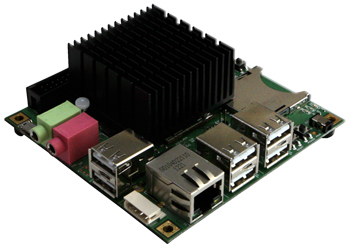
\includegraphics[width=0.7\textwidth]{figs/odroid.jpg}
    \caption{Image of the Hardkernel ODROID-X2 from the Hardkernel ODROID-X2
    product page \cite{hardkernelodroidx2}.}
    \label{fig:odroidx2}
\end{figure}

The ODROID-X2 developer platform \cite{hardkernelodroidx2} is used as a
reference hardware for all experiments in this thesis. An image of the platform
is shown in \autoref{fig:odroidx2}. Its core voltage is easily accessible on an
attached daughter board right beneath the heat sink, making it easy to conduct
power measurements. The board is equipped with a Samsung Exynos 4412 ``Prime'',
a modern System-on-Chip featuring four ARM Cortex-A9 CPU cores, Mali-400 GPU and
2~GB of on-chip DRAM. The Cortex-A9 is one of ARM's mid-to-high-range application
processors. It features an out-of-order dual-issue speculative RISC core, and it
is clearly designed with emphasis on energy efficiency. This processor is
primarily found in low-powered embedded devices with some performance demands,
typically smartphones and tablets.

\begin{figure}[bht]
    \centering
    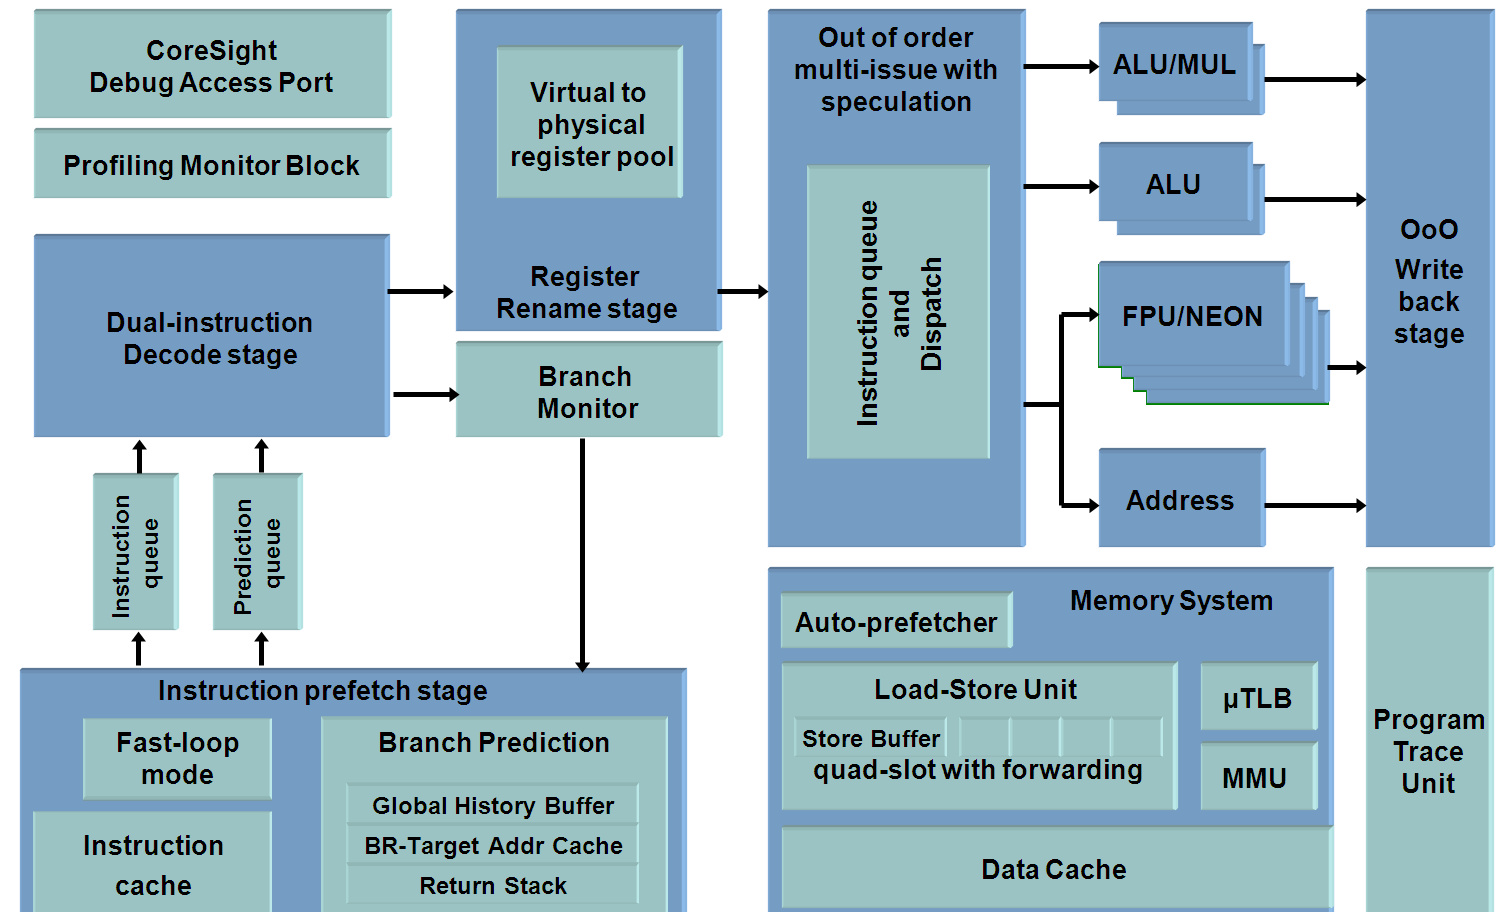
\includegraphics[width=\textwidth]{figs/A9-Pipeline-hres.jpg}
    \caption{A brief overview of the Cortex-A9 Pipeline, figure from the ARM
    Cortex-A9 Whitepaper \cite{a9whitepaper}.}
    \label{fig:a9arch}
\end{figure}

\autoref{fig:a9arch} shows an overview of the ARM Cortex-A9 architectural
structure. It features an out-of-order multi-issue module right after the decode
stage. This module can do speculative issue and schedules two arithmetic
operations per cycle. It also features a multiplexed lane for address operations
and floating point operations (the \emph{NEON} FPU). In this experiment, a
4-core variant of the processor was used, but 3 of the cores were disabled to
ease both the measurement and the simulation process. \autoref{tab:hwspecx2}
enumerates the most important properties of the SoC.


\rowcolors{2}{gray!25}{white}
\begin{table}
    \centering
    \begin{tabular}{|c|l|}
        \rowcolor{gray!25}
        \hline
        Manufacturer   & Hardkernel \\
        Platform       & ODROID-X2 \\
        SoC            & Samsung Exynos 4412 ``Prime'' \\
        CPU Core       & ARM Cortex-A9 (r3p0) \\
        Number of Cores& 4 \\
        Clock Frequency& 1.7~GHz \\
        Core Voltage   & 1.3~V \\
        L1 Cache       & Dual 32~KB \\
        L2 Cache       & 1~MB \\
        Main Memory    & 2~GB LP-DDR2 880~MHz \\
        \hline
    \end{tabular}
    \caption{Hardware specifications ODROID-X2.}
    \label{tab:hwspecx2}
\end{table}

